% This is a Basic Assignment Paper but with like Code and stuff allowed in it, there is also url, hyperlinks from contents included. 

\documentclass[11pt]{article}

% Preamble

\usepackage[margin=1in]{geometry}
\usepackage{amsfonts, amsmath, amssymb}
\usepackage{fancyhdr, float, graphicx}
\usepackage[utf8]{inputenc} % Required for inputting international characters
\usepackage[T1]{fontenc} % Output font encoding for international characters
\usepackage{fouriernc} % Use the New Century Schoolbook font
\usepackage[nottoc, notlot, notlof]{tocbibind}
\usepackage{listings}
\usepackage{xcolor}
\usepackage{blindtext}
\usepackage{hyperref}
\hypersetup{
    colorlinks=true,
    linkcolor=black,
    filecolor=magenta,      
    urlcolor=cyan,
    pdfpagemode=FullScreen,
    }

\definecolor{codegreen}{rgb}{0,0.6,0}
\definecolor{codegray}{rgb}{0.5,0.5,0.5}
\definecolor{codepurple}{rgb}{0.58,0,0.82}
\definecolor{backcolour}{rgb}{0.95,0.95,0.92}

\lstdefinestyle{mystyle}{
    backgroundcolor=\color{backcolour},   
    commentstyle=\color{codegreen},
    keywordstyle=\color{magenta},
    numberstyle=\tiny\color{codegray},
    stringstyle=\color{codepurple},
    basicstyle=\ttfamily\footnotesize,
    breakatwhitespace=false,         
    breaklines=true,                 
    captionpos=b,                    
    keepspaces=true,                 
    numbers=left,                    
    numbersep=5pt,                  
    showspaces=false,                
    showstringspaces=false,
    showtabs=false,                  
    tabsize=2
}

\lstset{style=mystyle}

% Header and Footer
\pagestyle{fancy}
\fancyhead{}
\fancyfoot{}
\fancyhead[L]{\textit{\Large{Internet of Things Lab Assignment 4}}}
\fancyhead[R]{\textit{\Large{Krishnaraj}}}
\fancyfoot[C]{\thepage}
\renewcommand{\footrulewidth}{1pt}



% Other Doc Editing
% \parindent 0ex
%\renewcommand{\baselinestretch}{1.5}

\begin{document}

\begin{titlepage}
	\centering

	%---------------------------NAMES-------------------------------

	\huge\textsc{
		MIT World Peace University
	}\\

	\vspace{0.75\baselineskip} % space after Uni Name

	\LARGE{
		Internet of Things\\
		Second Year B. Tech, Semester 2
	}

	\vfill % space after Sub Name

	%--------------------------TITLE-------------------------------

	\rule{\textwidth}{1.6pt}\vspace*{-\baselineskip}\vspace*{2pt}
	\rule{\textwidth}{0.6pt}
	\vspace{0.75\baselineskip} % Whitespace above the title



	\huge{\textsc{
			Traffic Light Simulation using Raspberry Pi
		}} \\



	\vspace{0.5\baselineskip} % Whitespace below the title
	\rule{\textwidth}{0.6pt}\vspace*{-\baselineskip}\vspace*{2.8pt}
	\rule{\textwidth}{1.6pt}

	\vspace{1\baselineskip} % Whitespace after the title block

	%--------------------------SUBTITLE --------------------------	

	\LARGE\textsc{
		Assignment 4
	} % Subtitle or further description
	\vfill

	%--------------------------AUTHOR-------------------------------

	Prepared By
	\vspace{0.5\baselineskip} % Whitespace before the editors

	\Large{
		Krishnaraj Thadesar \\
		Cyber Security and Forensics\\
		Batch A2, PA 20
	}


	\vspace{0.5\baselineskip} % Whitespace below the editor list
	\today

\end{titlepage}


\tableofcontents
\thispagestyle{empty}
\clearpage

\setcounter{page}{1}

\section{Aim}
Consider a suitable scenario of traffic signalling considering a crossroad and demonstrate the working of traffic lights using Raspberry Pi.
\section{Objectives}
\begin{itemize}
	\item To simulate a traffic signal using Raspberry Pi.
	\item To demonstrate the working of traffic lights using Raspberry Pi.
\end{itemize}

\section{Component List}
\begin{table}[H]
	\begin{tabular}{|l|l|}
		\hline
		\textbf{Equipment Name}   & \textbf{Quantity} \\ \hline
		Raspberry Pi Model 3 B    & 1                 \\ \hline
		LEDs - Green, Yellow, Red & 3                 \\ \hline
	\end{tabular}
\end{table}
\section{Theory}

In this project, the Raspberry Pi will be used to control the traffic lights, which will be represented using LEDs. The project will involve programming the Raspberry Pi to alternate the lights in a manner similar to real-world traffic lights. This will require knowledge of programming languages such as Python, as well as knowledge of the GPIO pins on the Raspberry Pi, which are used to interface with external components.\\

IoT concepts that may be involved in this project include the use of sensors to detect the presence of vehicles or pedestrians, which could be used to control the timing of the traffic lights. For example, if a sensor detects a vehicle waiting at a red light, it could signal the Raspberry Pi to shorten the duration of the red light and increase the duration of the green light to allow the vehicle to proceed. This concept is known as "smart traffic management" and is an example of how IoT can be used to improve transportation infrastructure.\\

Additionally, the Raspberry Pi could be connected to a network and communicate with other devices in the IoT ecosystem. For example, it could send data about traffic flow to a central server, which could be used to analyze traffic patterns and make decisions about traffic management. This is an example of how IoT can be used to gather and analyze large amounts of data to improve decision-making processes.\\

Overall, this project is an example of how IoT can be used to create innovative solutions for real-world problems. By simulating traffic lights using a Raspberry Pi, students can learn valuable programming and electronics skills while also gaining a deeper understanding of IoT concepts such as smart traffic management and data analysis.\\

\section{Platform}
\textbf{Operating System}: Arch Linux x86-64 \\
\textbf{IDEs or Text Editors Used}: Thonny\\
\textbf{Compilers} : Python 3.10 in Raspberry Pi.

\section{Circuit Diagram}
\begin{figure}[H]
	\centering
	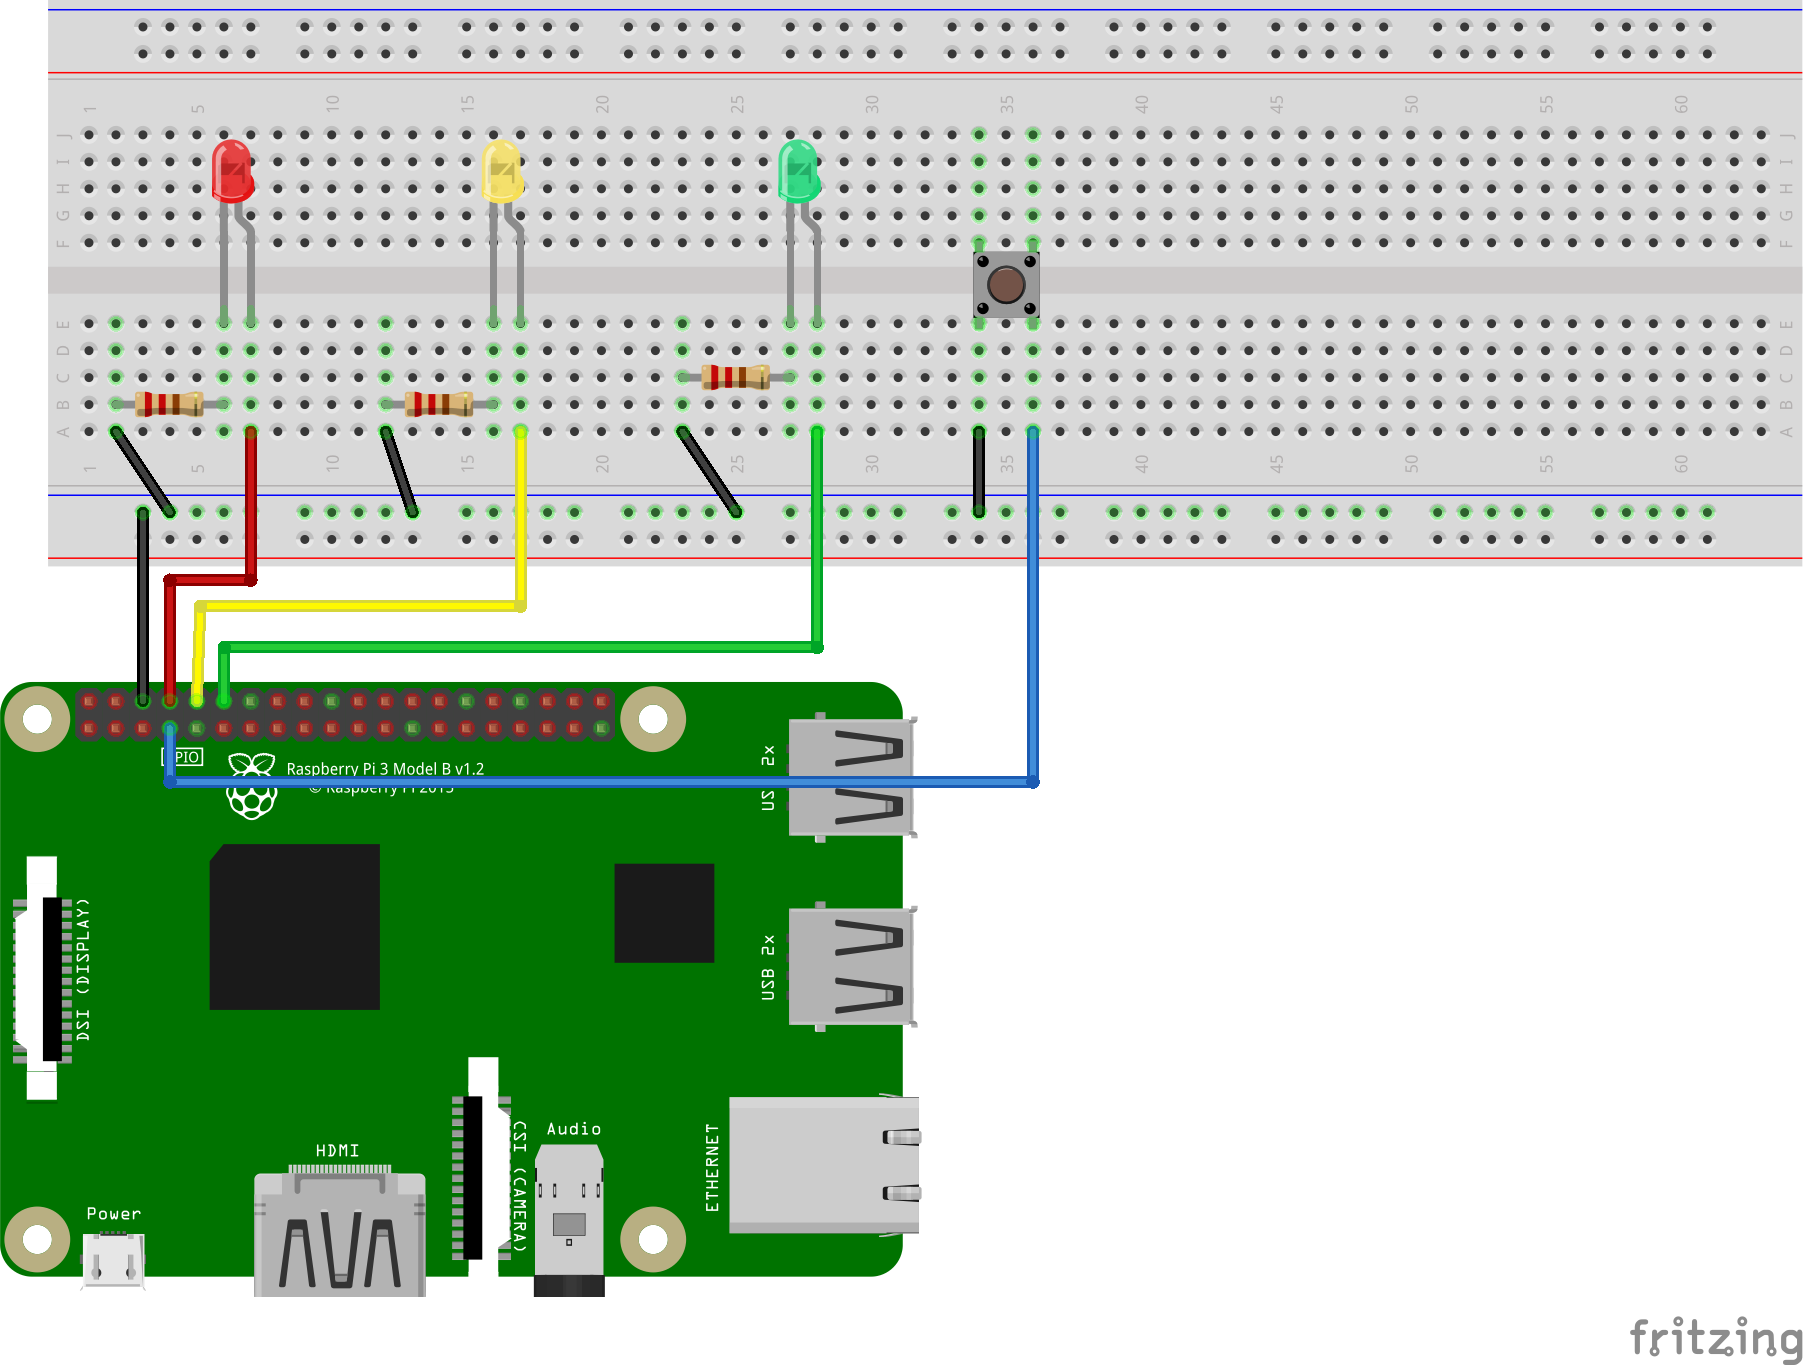
\includegraphics[width=.45\textwidth]{traffic-signal_bb.png}
	\caption{Circuit Diagram for Traffic Signal}
\end{figure}


\section{Code}
\begin{lstlisting}[language=python]

	from gpiozero import LED
	from gpiozero import Button
	from gpiozero import TrafficLights
	import time
	
	# TrafficLights(red, amber, green)
	lights = TrafficLights(25, 8, 7)
	button = Button(21)
	
	
	def traffic(hour):
	  t = time.localtime()
	  h = t.tm_hour
	  lights.amber.on()
	  time.sleep(2)
	  lights.amber.off()
	  if (21 > h and 6 < h):
		lights.green.on()
		time.sleep(5)
		lights.green.off()
	  else:
		lights.red.on()
		time.sleep(5)
		lights.red.off()
	
	def wakey(hour, min):
	  cnt = 0
	  while cnt < 10:
		if (hour == 6 and min == 40):
		  lights.green.on()
		  lights.red.on()
		  lights.amber.on()
		  time.sleep(1)
		  lights.green.off()
		  lights.red.off()
		  lights.amber.off()
		  time.sleep(1)
		cnt+=1
	
	while True:
	  w = time.localtime()
	  wakey(w.tm_hour, w.tm_min)
	  button.when_pressed = traffic
\end{lstlisting}
\section{Conclusion}
Thus, we have successfully simulated a traffic signal using Raspberry Pi.
\clearpage

\section{FAQ}

\begin{enumerate}
	\item Raspberry Pi Model 3 B: \\
	      The Raspberry Pi has a total of 40 pins, including 26 GPIO (General Purpose Input/Output) pins, 3.3V and 5V power pins, and ground pins. The pinout diagram for the Raspberry Pi 3 B can be found on the official Raspberry Pi website.

	      \begin{itemize}
		      \item Pin 1: 3.3V
		      \item Pin 2: 5V
		      \item Pin 3: GPIO 2
		      \item Pin 4: 5V
		      \item Pin 5: GPIO 3
		      \item Pin 6: Ground
		      \item Pin 7: GPIO 4
		      \item Pin 8: GPIO 14
		      \item Pin 9: Ground
		      \item Pin 10: GPIO 15
		      \item Pin 11: GPIO 17
		      \item Pin 12: GPIO 18
		      \item Pin 13: GPIO 27
		      \item Pin 14: Ground
		      \item Pin 15: GPIO 22
		      \item Pin 16: GPIO 23
		      \item Pin 17: 3.3V
		      \item Pin 18: GPIO 24
		      \item Pin 19: GPIO 10
		      \item Pin 20: Ground
		      \item Pin 21: GPIO 9
		      \item Pin 22: GPIO 25
		      \item Pin 23: GPIO 11
		      \item Pin 24: GPIO 8
		      \item Pin 25: Ground
		      \item Pin 26: GPIO 7
		      \item Pin 27: ID SD
		      \item Pin 28: ID SC
		      \item Pin 29: GPIO 5
		      \item Pin 30: Ground
		      \item Pin 31: GPIO 6
		      \item Pin 32: GPIO 12
		      \item Pin 33: GPIO 13
		      \item Pin 34: Ground
		      \item Pin 35: GPIO 19
		      \item Pin 36: GPIO 16
		      \item Pin 37: GPIO 26
		      \item Pin 38: GPIO 20
		      \item Pin 39: Ground
		      \item Pin 40: GPIO 21
	      \end{itemize}

	\item LED: \\


	      LEDs are diodes that emit light when an electric current passes through them. They are used as indicator lamps in many devices, and are increasingly used for lighting. \\

	      The LED is based on the semiconductor diode. When a diode is forward biased (switched on), electrons are able to recombine with holes within the device, releasing energy in the form of photons.\\

	      This effect is called electroluminescence and the color of the light (corresponding to the energy of the photon) is determined by the energy band gap of the semiconductor. LEDs are typically small (less than 1 mm2) and integrated optical components may be used to shape the radiation pattern.

	      The Pins are:
	      \begin{itemize}
		      \item Anode
		      \item Cathode
	      \end{itemize}

\end{enumerate}

\end{document}